% The step mappings rho and pi on lanes [FIPS 202, §3.2.2, Table 2; §3.2.3]: rho rotates lane
% (x, y) by the offset shown (taken mod w); pi moves the lane at ((x + 3y) mod 5, x) to (x, y).
% Original drawing for the Hash library.
\documentclass[tikz,border=6pt]{standalone}
\usepackage[T1]{fontenc}
\usepackage{lmodern}
% Shared style for the Hash diagrams.
% Palette: Okabe–Ito (colour-blind safe). Every diagram is drawn on an opaque white card so it
% stays legible on dark page themes.
\usetikzlibrary{arrows.meta,positioning,calc,fit,backgrounds}
\definecolor{hsblue}{HTML}{0072B2}
\definecolor{hsorange}{HTML}{E69F00}
\definecolor{hsgreen}{HTML}{009E73}
\definecolor{hsvermilion}{HTML}{D55E00}
\definecolor{hspurple}{HTML}{CC79A7}
\definecolor{hsink}{HTML}{1F2933}
\tikzset{
  >={Stealth[length=2.2mm]},
  every node/.style={font=\sffamily\small, text=hsink},
  wire/.style={draw=hsink, line width=0.6pt, ->},
  reg/.style={draw=hsink, line width=0.6pt, fill=hsblue!12, minimum width=9mm, minimum height=7mm},
  fn/.style={draw=hsink, line width=0.6pt, fill=hsorange!25, rounded corners=2pt, minimum width=10mm, minimum height=6mm},
  input/.style={draw=hsink, line width=0.6pt, fill=hsgreen!20, minimum width=9mm, minimum height=6mm},
  add/.style={circle, draw=hsink, line width=0.6pt, fill=white, inner sep=0pt, minimum size=5mm, font=\sffamily\bfseries},
  card/.style={fill=white, rounded corners=4pt},
}

\begin{document}
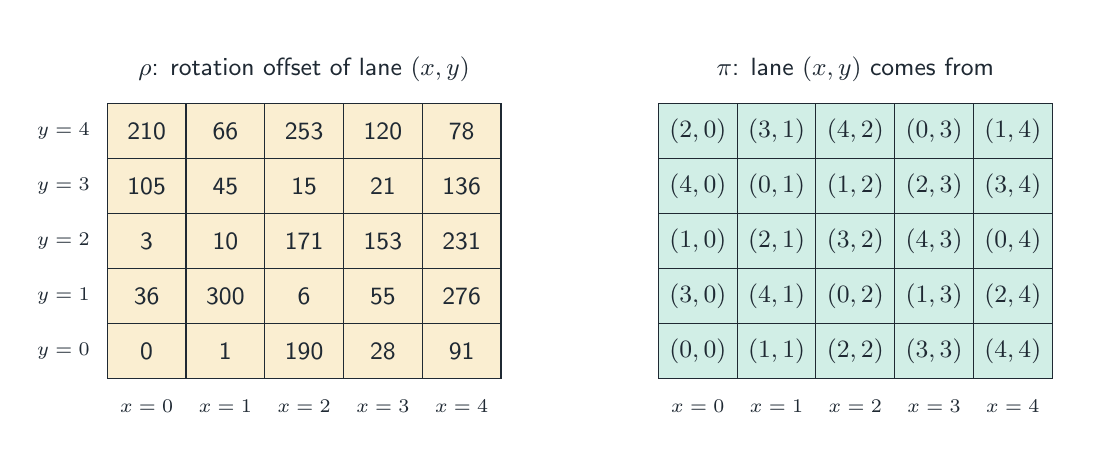
\begin{tikzpicture}[cell/.style={draw=hsink, line width=0.4pt, minimum width=10mm, minimum height=7mm, inner sep=0pt, font=\sffamily\small}]
  \def\s{1.0}
  \def\t{0.7}
  % rho offsets, indexed (x, y), y increasing upwards.
  \foreach \row [count=\yy from 0] in {{0,1,190,28,91},{36,300,6,55,276},{3,10,171,153,231},{105,45,15,21,136},{210,66,253,120,78}} {
    \foreach \v [count=\xx from 0] in \row {
      \node[cell, fill=hsorange!18] (r\xx\yy) at (\xx*\s, \yy*\t) {\v};
    }
  }
  \foreach \xx in {0,...,4} \node[font=\scriptsize] at (\xx*\s, -0.7) {$x=\xx$};
  \foreach \yy in {0,...,4} \node[font=\scriptsize, anchor=east] at (-0.6, \yy*\t) {$y=\yy$};
  \node[font=\sffamily\small, anchor=south] at (2*\s, 4*\t+0.5) {$\rho$: rotation offset of lane $(x,y)$};
  % pi: the source lane of each target lane.
  \foreach \xx in {0,...,4} \foreach \yy in {0,...,4} {
    \pgfmathtruncatemacro{\sx}{mod(\xx + 3*\yy, 5)}
    \node[cell, fill=hsgreen!18] (p\xx\yy) at (7.0+\xx*\s, \yy*\t) {$(\sx,\xx)$};
  }
  \foreach \xx in {0,...,4} \node[font=\scriptsize] at (7.0+\xx*\s, -0.7) {$x=\xx$};
  \node[font=\sffamily\small, anchor=south] at (7.0+2*\s, 4*\t+0.5) {$\pi$: lane $(x,y)$ comes from};
  \begin{scope}[on background layer]
    \coordinate (e1) at (-1.3,-0.9);
    \coordinate (e2) at (11.6,3.9);
    \node[card, fit=(r00)(p44)(e1)(e2), inner sep=6pt] {};
  \end{scope}
\end{tikzpicture}
\end{document}
